
\documentclass{scrartcl}

\usepackage{graphicx}
\usepackage[x11names, dvipsnames*, svgnames]{xcolor}
\setlength{\fboxsep}{.05\linewidth}
\usepackage[hyperindex=false, pdfpagelabels,
pageanchor, hyperfootnotes=false, bookmarksopen,
pdfpagemode=UseOutlines]{hyperref}

\usepackage{mathspec}
\usepackage{fontspec}
\usepackage{xunicode}
\usepackage[no-sscript]{xltxtra}

\setmainfont[Mapping=tex-text,  Scale=1.03, ItalicFeatures={SmallCapsFont=AlegreyaSC-Italic}]{Alegreya}
\setsansfont[Mapping=tex-text, Scale=1.03]{Alegreya Sans}

\usepackage{polyglossia}
\setdefaultlanguage{english}

\usepackage{microtype}
\usepackage{xspace}

\setlength{\parindent}{0pt}
\sloppy


\author{Sebastian Meisel}

\date{27. Januar 2020}

\title{Einführung in LaFiC}

\begin{document}

\maketitle


\colorbox{red}{\parbox{\linewidth}{%%
\begin{center}
\textcolor{white}{%%
LaFiC ist im Alpha-Status und ist nicht für produktives Arbeiten geeignet!}
\end{center}

}
}

{LaFiC bedeutet \textit{layout and format in comments}, also „Layout
und Format in Kommentaren“, denn sämtliche Formatierungen
werden in LAFIC in Kommentarzeilen ausgeführt. Das
ermöglicht eine \emph{vollständige} Trennung von Inhalt und
Gestalt.\\}

\section{Warum LaFiC}

{Ich arbeite nun schon viele Jahre mit \LaTeX\  / \XeLaTeX\ . Ich
schreibe vor allem Prosa (ganz frei von mathematischen
Formeln). Dabei fand ich es zum Teil störend, dass ich immer
erst mit der Preamble beginnen muss und nicht einfach
losschreiben kann.\\}

{Daraufhin probierte ich markdown / multimarkdown aus. Dabei
störte mich aber, dass es sehr unflexible ist. Außerdem ist
die Syntax an manchen Stellen etwas kryptisch, was mich
störte. Außerdem funktionieren die erstellten \LaTeX\ -Dateien
zwar irgendwie, sind aber auch sehr kryptisch aufgebaut.\\}

{Außerdem hatte ich immer die Worte meines Vaters im Ohr, der
sagte, er wolle am liebsten, wie einst mit der
Schreibmaschiene losschreiben können und dennoch ein
ordentliches Ergebnis bekommen.\\}

{Als letzte Motivation kam hinzu, dass ich immer wieder
darüber nachdachte, wie sich Inhalts- und
Gestaltungselemente des Textes noch sauberer trennen lassen,
als dies mit bisherigen Ansätzen möglich ist.\\}

{Mit LaFiC kann ich direkt losschreiben und bekomme von
anfang an ein ordentlich strukturiertes Ergebnis als Html-
und (Xe)LaTeX-\footnote{Die Standard-Vorlagen, die LaFiC nutzt basieren auf \XeLaTeX\ , da ich immer in Utf-8 schreibe. Die Nutzung von \LaTeX\  sollte aber auch möglich sein.}\xspace Datei, wodurch auch eine Ausgabe als Pdf
möglich ist.\\}

{Die eigentliche Formatierung geschieht erst im
Anschluss. Als mein eigener Lektor gehe ich durch den Text
und formatiere ihn mit für Menschen lesbaren und
verständlichen Kommentaren.\\}

\part{Installation und Benutzung}

\section{Vorraussetzungen}

{LaFiC setzt Perl > 5.10.1 vorraus (getestet unter Perl 5.26.1).\\}

{Das Standard \LaTeX\ -Template setzt eine aktuelle
\XeLaTeX\ -Installation sowie graphicx, hyperref, microtype und
xspace voraus.\\}

{Die Gnu-Emacs-Einbindung wurde unter Gnu Emacs 25.2.2 getestet.\\}

{\texttt{lafic2pdf} setzt zudem latexmk (getestet mit Version 4.41) vorraus.\\}

{\texttt{lafic2html} benötigt \texttt{latexmk} und \texttt{pdf2svg} (getestet mit
Version 0.2.3-1).\\}

\section{Installation}
\label{Installation}

{Holen Sie den Quelltext von \href{https://github.com/SebastianMeisel/lafic}{github}:\\}

\begin{verbatim}
git clone https://github.com/SebastianMeisel/lafic.git
\end{verbatim}


{Fügen Sie den Pfad zu \$PATH Umgebungsvariable hinzu:\\}

\begin{verbatim}
export PATH=${PATH}:~/lafic
\end{verbatim}


{Zur Nutzung des Major Modes in Emacs, kopieren (oder
verlinken) die Dateien \texttt{lafic-mode.el} und
\texttt{lafic-german-keywords.el} in ein Verzeichnis in Ihrem
\texttt{load-path}. Fügen Sie folgende Zeilen in Ihre Init-Datei
(\textasciitilde /.emacs) ein:\\}

\begin{verbatim}
(setq lafic-use-german t)
(require 'lafic-mode)
\end{verbatim}


{Wenn Sie keine Unterstützung von deutschen Schlüsselwörtern
wünschen oder benötigen, lassen Sie die erste Zeile weg.\\}

\section{Nutzung}

{Momentan besteht die LaFiC-Distribution aus drei
Skripten. Der Aufruf erfolgt jeweils analog:\\}

\begin{verbatim}
# lafic2html Datei.lafic
# lafic2tex Datei.lafic
# lafic2pdf Datei.lafic
\end{verbatim}


{Letzteres ruft zuerst \texttt{lafic2tex} und \texttt{latexmk} auf.\\}

{Durch den Aufruf dieser drei Skripte würden folgende Dateien
erstellt:\\}

\begin{verbatim}
Datei.html
Datei.tex
Datei.pdf
\end{verbatim}


\section{Nutzung des LaFiC-Major-Modes in GNU Emacs}

{Nachdem Sie \texttt{lafic-mode.el} wie oben (siehe \nameref{Installation}\xspace )
beschrieben in Emacs eingebunden haben, wird der
LaFiC-Major-Mode beim Öffnen einer Datei mit der Endung
\texttt{*.lafic} aktiviert.\\}

{Dadurch stehen eine einfache Syntaxhervorhebung und einige
Tastenkürzel zur Verfügung. Als Prefix wird dabei jewweil
\texttt{C-c} verwendet. Die Tastenkürzel orientieren sich an AUCTeX,
sodass man gut zurecht kommen sollte, wenn man damit schon
gearbeitet hat.\\}

\part{Schreiben mit LaFiC}

\section{Zeilen und Absätze}

{Der Inhalt wird durch die Unterscheidung von \emph{Zeilen} und
\emph{Absätzen} gegliedert.\\}

{Dabei besteht der Unterschied nicht so sehr in der
Länge. Vielmehr unterscheiden sich Zeilen von Absätze
dadurch, dass sie kein Satzschlusszeichen \emph{(., ?, !, :)}.
Wenn nicht anders festgelegt, werden sie als Überschriften
interpretiert.\\}

{Die erste \emph{Zeile} wird als Titel interpretiert und zu \textbackslash title
umgewandelt, wenn die Datei in \LaTeX\  umgewandelt wird, bei
\textsc{Html}-Ausgabe wird es in <h1> umgewandelt.\\}

{Weitere \emph{Zeilen} werden in <h3> (\textsc{Html}) oder \textbackslash section
(LaTeX) umgewandelt, wenn es nicht anders angegeben wird.\\}

{Auf diese Weise können einfache Texte ganz ohne Formatierung
gegliedert werden.\\}

\section{Kommentare}

{Man kann im Text jeder Zeit Kommentare einführen in dem man einen Absatz einfügt, der mit zwei \%-Zeichen beginnt:\\}

\begin{verbatim}
  %% Dies ist ein Kommentar.

  %% Dies ist ein längerer Kommentar. Es ist wichtig, dass
  %% Kommentare immer durch eine Leerzeile vom eigentlichen
  %% Inhalt getrennt sind.
\end{verbatim}




\section{Formatierte Absätze}

{Absätze können formatiert werden, in dem eine Zeile
vorangestellt wird, die mit einem \%-Zeichen beginnt dem ein
Schlüsselwort folgt. Ist das Schlüsselwort bekannt, wird
die entsprechende Umgebung (LaTeX), bzw. der entsprechende
Block (Html) ausgegeben. Ansonsten dient das Schlüsselwort
(umgewandelt in Kleinschreibung) als Name der Umgebung
(LaTeX), bzw. eines <div>-Blocks (Html).\\}

\begin{verbatim}
  % Zentriert
  Dieser Absatz ist zentriert.
\end{verbatim}


\begin{center}
Dieser Absatz ist zentriert.
\end{center}


{Folgen zwei Absätze mit dem selben Schlüsselwort
hintereinander, werden sie in einer Umgebung / einem Block
zusammengefasst.\\}

\begin{verbatim}
  % Zitat
  Dies ist ein Zitat.

  % Zitat
  Hier geht das Zitat weiter.
\end{verbatim}


{Wird zu:\\}

\colorbox{gray!75}{\parbox{\linewidth}{%%
\begin{quote}
\centering%%
Dies ist ein Zitat.

Hier geht das Zitat weiter.
\end{quote}

}
}

{Zur Zeit werden folgende Schlüsselworte unterstützt:\\}

\begin{itemize}
\item \texttt{„Zitat“} für quote-Umgebung / <blockquote>-Block.
\item \texttt{„Langzitat“} / LZitat für quotation-Umgebung / <blockquote>-Block.
\item \texttt{„Zentriert“} / Z für center-Umgebung / <div class=\texttt{„center“}>-Block mit text-align=\texttt{„center“}
\item „Verbatim“ für verbatim-Umgebung / <pre>-Block
\end{itemize}


\section{Formatierte Zeilen}

{Zeilen werden auf die gleiche Weise formatiert, nur werden sie in Makros (LaTeX) oder <span>-Ids (Html) umgewandelt. Zeilen sind in der Regel Überschriften.\\}

\begin{verbatim}
    % Unterunterabschnitt
    Das ist ein Unterunterabschnitt
\end{verbatim}


\subsubsection{Dies ist ein Unterunterabschnitt}

{Folgende Schlüsselwörter werden zur Zeit unterstützt:\\}

\begin{itemize}
\item \texttt{„Überschrift“} für \textbackslash addsec / <h3>
\item \texttt{„Titel“}, „Überschrift1“  für \textbackslash title / <h1>
\item \texttt{„Teil“} / „Überschrift2“ für \textbackslash part / <h2>
\item \texttt{„Kapitel“} für \textbackslash chapter / <h2>\footnote{Wird nicht von der Standard-Vorlage unterstützt. Es muss eine \LaTeX\ -Klasse verwendet werden, die \textbackslash chapter unterstützt.}\xspace  
\item \texttt{„Abschnitt“}, „Überschrift3“ für \textbackslash section / <h3>
\item \texttt{„Unterabschnitt“} / „Überschrift4“ für \textbackslash subsection / <h4>
\item \texttt{„Unterunterabschnitt“} / „Überschrift5“ für \textbackslash subsubsection / <h5>
\item \texttt{„Absatz“} / „Überschrift6“ für \textbackslash paragraph / <h6>
\end{itemize}


\subsection{Metadaten}

{Metadaten können als formatierte Zeilen angegeben werden:\\}

\begin{verbatim}
  % Autor
  Max Mustermann

  % Datum
  Sankt-Nimmerleins-Tag
\end{verbatim}


{Dies sind zur Zeit auch die beiden einzigen Schlüsselwörter,
wobei alternativ „\texttt{von}“ und „\texttt{am}“ zur Verfügung stehen.\\}

\section{Textformatierung im Absatz}

{Wörter und Textabschnitte in einem Absatz werden in einem
Block nach dem Absatz formatiert. Jede Zeile beginnt mit
einem »\texttt{\%}« gefolgt von:\\}

\begin{enumerate}
\item dem Wort
\item dem ersten und letzten Wort den Abschnittes,
  getrennt durch 3~Punkte, bzw. durch »…«.
\end{enumerate}


{Sie sind durch einen Doppelpunkt getrennt.\\}

\begin{verbatim}
  Hallo gute alte Welt!
  % Hallo: fett
  % al…lt: hervorheben
\end{verbatim}


{wird zu:
\textbf{Hallo} gute \emph{alte Welt}!\\}

{Folgende Schlüsselworte werden zur Zeit unterstützt:\\}

\begin{itemize}
\item \texttt{„fett“} für \textbackslash textbf / <b>
\item \texttt{„hervorheben“} für \textbackslash emph / <em>
\item \texttt{„kursiv“} für \textbackslash textit / <i>
\item \texttt{„Schreibmaschiene“} oder \texttt{„nicht proportional“} für \textbackslash texttt / <span class=‚tt‘>
\item \texttt{„Kapitälchen“} für \textbackslash textsc / <span class=‚sc‘>
\item \texttt{„hochgestellt“} für \textbackslash textsuperscript / <sup>
\item \texttt{„tiefgestellt“} für \textbackslash textsubscript / <sub>
\end{itemize}


{Unbekannte Schlüsselworte werden in Makros (LaTeX) oder
<span>-Elemente (Html) umgewandelt.\\}

{Einige Schlüsselworte benötigen ein zweites Argument, dass
nach einem zweiten Doppelpunkt angefügt wird:\\}

\begin{verbatim}
  Die Welt ist grün!
  % grün: Farbe: rot
\end{verbatim}


{Wird zu:
Die Welt ist \textcolor{red}{grün}!\\}

{Folgende solcher Schlüsselworte werden zu Zeit unterstützt:\\}

\begin{itemize}
\item „url“ oder „link“ für \textbackslash href / <a href=‚{[url‘]}>
\item „siehe“ für \textbackslash nameref / <a href='\#{[label]}‘> 
\item „Fußnote“ für  \textbackslash footnote / <a class=‚fn‘ href=‚xfn{[x]}‘\footnote{In Html-Dokumenten werden Fußnoten in einer <ol>-Liste in einem <div id=„footnote“>-Container am Ende des Dokumentes dargestellt. Die einzelnen Fußnoten stehen in einem <li id=„fn{[x]}“>-Element.}\xspace >
\item „Farbe“ für \textbackslash textcolor / <span style=‚color: {[color]}‘>
\end{itemize}


\section{Parameter}

{Es ist weiterhin möglich einer Zeile oder einem Absatz
zusätzliche Parameter hinzuzufügen. Die geschieht äquivalent
zu Formatierung im Absatz, nur dass ein Ist-gleich-Zeichen
statt des Doppelpunktes gesetzt wird:\\}

\begin{verbatim}
  Dieser Text ist rot auf blauem Untergrund und
  rechtsbündig.
  % Hintergrundfarbe = blau
  % Farbe = rot
  % Ausrichtung = rechtsbündig
\end{verbatim}


{wird zu:\\}

\colorbox{PaleTurquoise1}{\parbox{\linewidth}{%%
{\raggedleft%%
\textcolor{red}{%%
Dieser Text ist rot auf blauem Untergrund und
rechtsbündig.}\\}
}
}

{Folgende Parameter werden derzeit unterstützt:\\}

\begin{itemize}
\item „Name“, „Bezeichnung“ oder  „Label“ für \textbackslash label / <?? id=„{[id]}“> that is
  referred to by the „see“ keyword.
\item „Hintergrund“ für \textbackslash colorbox / <div style=‚background: {[color]}‘>.
\item „Farbe“ für \textbackslash textcolor / <div style=‚color: {[color]}‘>.
\item „Ausrichtung“ :  „rechtsbündig“ für \textbackslash raggedleft,  „zentriert“ für \textbackslash centering oder „linksbündig“ für
  \textbackslash raggedright / <div style=‚text-align: {[align]}‘>.
\end{itemize}


\section{Listen}

{List sind das Einzige, das eine Art Auszeichnung benötigt:
Sie müssen jeden Punkt in der List mit einem der folgenden
Zeichen beginnen:~\texttt{–, *, +, -}. Dabei spielt es keine Rolle,
welches Sie wählen. Sie können Zeilen einrücken, aber das
beeinflusst das Layout nicht.\\}

\begin{verbatim}

* Top 1.
- Top 2.
\end{verbatim}


\begin{itemize}
\item Top 1.
\item Top 2.
\end{itemize}


{Für Listen mit mehreren Ebenen haben Sie zwei Möglichkeiten,
die Ebene zu wechseln: Die reine LaFiC-Stil wäre, einen
neuen Abschnitt einzufügen und dahinter eines der
Schlüsselworte \texttt{»\% Level+«} oder \texttt{»\% Level-«} anzuhängen.\\}

\begin{verbatim}

  * Top 1.
  * Top 2.


  * Top 2a.
  * Top 2b.
  % level+
\end{verbatim}


\begin{itemize}
\item Top 1.
\item Top 2.

\begin{itemize}
\item Top 2a.
\item Top 2b.
\end{itemize}

\end{itemize}


{Die andere Möglichkeit ist die Liste in \emph{einem} Abschnitt zu
setzen und die Ebenenwechsel mit einem \texttt{Größer-}
bzw. \texttt{Kleiner-als-Zeichen} in einer ansonsten leeren Zeile anzuzeigen:\\}

\begin{verbatim}

  * Top 1.
  * Top 2.
  >
    * Top 2a.
    * Top 2b.
  <
  * Top 3
\end{verbatim}


\begin{itemize}
\item Top 1.
\item Top 2.
\begin{itemize}
\item Top 2a.
\item Top 2b.
\end{itemize}
\item Top 3
\end{itemize}


\section{Bilder}

{Die einfachste Möglichkeit ein Bild in eine LaFiC-Datei
einzubinden ist es, eine Zeile mit dem Namen des Bildes mit
einer der Dateiendungen png, jpg, jpeg oder gif einfügt:\\}

\begin{verbatim}
  Image.png
  % Breite = 50%
  % Ausrichtung = zentriert
\end{verbatim}


{\centering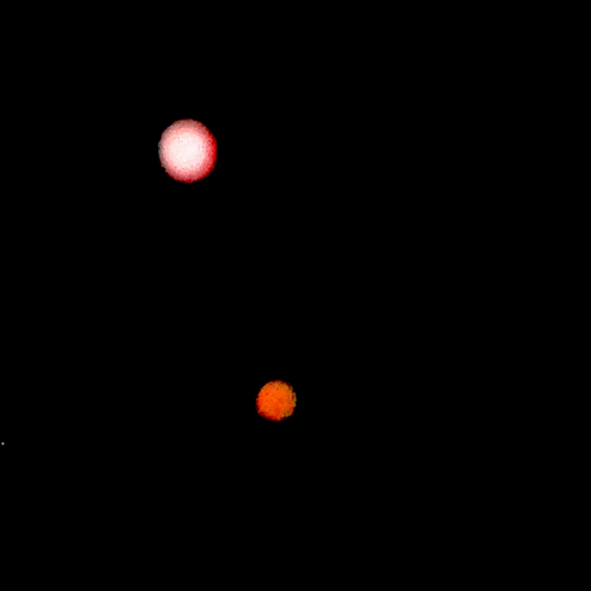
\includegraphics[width=.50\linewidth]{Image.png}\\}

{Zur Formatierung stehen folgende Parameter zur Verfügung:\\}

\begin{itemize}
\item Höhe
\item Breite
\item Ausrichtung
\end{itemize}


{Auf diese Art wird das Bild aber nicht als Flußelement
eingefügt. Dafür muss das Bild mit  \%Bild formatiert
werden.\\}

\begin{verbatim}
  % Bild
  Image.png
  % Höhe = 40%
  % Beschriftung = Mars and Moon
  % Name = bild1
  % Ausrichtung = rechtsbündig
\end{verbatim}


\begin{figure}[hbt]
\raggedleft%%
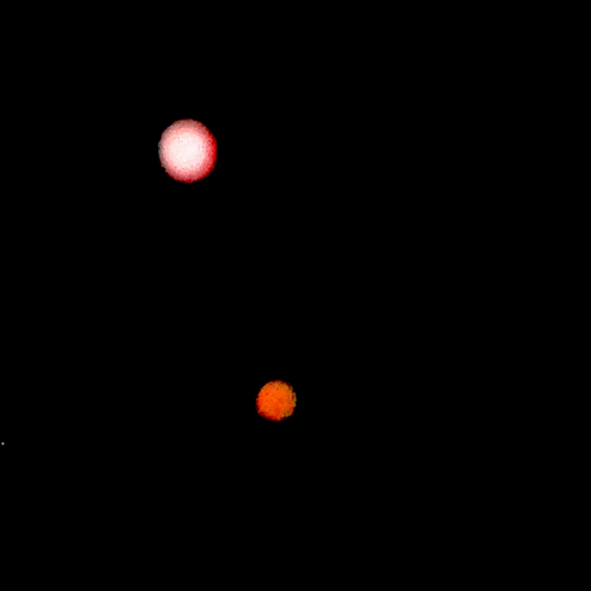
\includegraphics[height=.40\textheight]{Image.png}
\caption{Mars und Mond}
\label{bild1}
\end{figure}


{Damit stehen dann zwei weitere Parameter zur Verfügung:\\}

\begin{itemize}
\item Name
\item Beschriftung
\end{itemize}


\section{Farben}

{Folgende Farben werden zur Zeit als Argument für die
Parameter Farbe und Hintergrund unterstützt:\\}

\colorbox{gray!75}{\parbox{\linewidth}{%%
\begin{itemize}
\item grau
\item \textcolor{green}{grün}
\item \textcolor{LightYellow1}{gelb}
\item \textcolor{PaleTurquoise1}{blau}
\item \textcolor{red}{rot}
\item \textcolor{white}{weiß}
\end{itemize}

}
}

\section{Zeilenumbrüche}

{Zeilenumbrüche  innerhalb von Absätzen werden von LaFiC normalerweise entfernt. Um sie zu erhalten füge einfach \texttt{\% Zeilen umbrechen} hinter dem Absatz ein:\\}

\begin{verbatim}
  	     Geh mit mir.
	       Geh mir nah.
	       Geh mir zu Herzen und unter die Haut
	       % Geh: hervorheben
	       % Zeilen umbrechen
\end{verbatim}


{\emph{Geh} mit mir.\\
\emph{Geh} mich an.\\
\emph{Geh} mir auf die Nerven und hinter\emph{geh} mich~– wenn's sein muss!\\
Nur,\\
\emph{Geh} nicht!\\\\}

\section{LaTeX-Code}

{Es besteht die Möglichkeit reinen \LaTeX\ -Code wie folgt zu
nutzen:\\}

\begin{verbatim}
	% LaTeX
  	  $\left(\frac{1}{\sqrt{x}}\right)$  
	% Ausrichtung = center
\end{verbatim}


\centering%%
  $\left(\frac{1}{\sqrt{x}}\right)$
\part{Anpassung}

{LaFiC lässt sich auf verschiedene Weise anpassen.\\}

\section{Vorlagen}

{LaFiC nutzt Vorlagen. Diese liegen im Unterverzeichnis
\texttt{/templates} des LaFiC-Verzeichnisses und tragen die
Dateiendung .tmp.tex für \LaTeX\ -, bzw. .tmp.html für
Html-Dokumenten. Für deutschsprachige Projekte sollten die
Dateinamen auf \texttt{\_de\_DE} enden.\\}

{Sie können eigene Vorlagen erstellen und in diesem
Verzeichnis ablegen. LaFiC erwartet in \LaTeX\ -Vorlagen
dabei zumindest \texttt{graphicx} für das Einbinden von Bildern,
\texttt{hyperref} für die Nutzung von Links und \texttt{xcolor} mit den
optionen \texttt{x11names, dvipsnames* und svgnames}:\\}

\begin{verbatim}
	\usepackage{graphicx}
	\usepackage[x11names, dvipsnames*, svgnames]{xcolor}
	\usepackage[hyperindex=false, pdfpagelabels,
                    pageanchor, hyperfootnotes=false, bookmarksopen,
	    	    pdfpagemode=UseOutlines]{hyperref}
\end{verbatim}


{Die Vorlage wird aufgerufen, indem der Dateiname ohne
Dateiendung nach einem Prozentzeichen in die erste Zeile
eines Dokumentes eingefügt wird:\\}

\begin{verbatim}
	% Vorlage_de_DE
\end{verbatim}


{Außerdem ist es möglich Vorlagen für eine konkretes
Dokument zu erstellen, oder anzupassen. Solche Vorlagen
müssen im selben Verzeichnis wie das Dokument liegen und
denselben Dateinamen tragen:\\}

\begin{verbatim}
	$ ls -1
  	.
  	..
  	Beispiel.lafic
  	Beispiel.tmp.tex
  	Beispiel.tmp.html
\end{verbatim}


{In den Vorlagen müssen Platzhalter für die Metadaten und den
eigentlichen Dokumenttext enthalten sein.\\}

{In \LaTeX\ -Vorlagen sind das \%TITLE\% und \%TEXT\%:\\}

\begin{verbatim}
	\documentclass{article}
	 …
	%TITLE%
	\begin{document}
	%TEXT%
	\end{document}
\end{verbatim}


{In Html-Vorlagen heißen die Platzhalter <!-- TITLE~--> und
<!-- TEXT~-->:\\}

\begin{verbatim}
	<html>
       	<head>
		<!-- TITLE -->
       	</head>
       	<body>
		<!-- TEXT -->
       	</body>
	</html>
\end{verbatim}


\section{Für Fortgeschrittene: Eigene Schlüsselwörter}

{Wenn sie eigene \LaTeX\ -Umgebungen und Makros, sowie die dazu
passenden CSS-Klassen definieren, können Sie eigene
Schlüsselwörter benutzen.\\}

{Im Unterordner \texttt{examples} können Sie sich inspirieren lassen.\\}

\section{Stylesheets}

{Im Unterverzeichnis \texttt{/styles} befindet sich die Datei
\texttt{standard.css}. Sie enthält das Stylesheet für die
Standard-Html-Vorlagen von LaFiC. Sie können hier eigene
Stylesheets ablegen und Ihren Vorlagen verlinken. Zur Zeit
muss das Verzeichnis von Hand in das Arbeitsverzeichnis
kopiert oder dort verlinkt werden.\\}

\section{\texttt{lafic.config.pl}}

{In dieser Datei im LaFiC-Verzeichnis können Voreinstellungen
vorgenommen werden. Momentan gibt es nur zwei (mögliche)
Einträge:\\}

\begin{itemize}
\item \texttt{lang} für die Standardsprache. Statt dem Englisch wird hier
  zur Zeit nur \texttt{de\_DE} als Eintrag für die Deutsche Sprache
  unterstützt.
\item \texttt{author} ist Momentan die einzige Möglichkeit den Autor für
  ihre Dokumente zu setzen.
\end{itemize}


{Die Eintäge in dieser Datei sind Perlkonstrukte und müssen
in der Form:\\}

\begin{verbatim}
	Schlüssel => "Wert",
\end{verbatim}


{geschrieben werden. Bitte beachten sie das Komma am Ende der Zeile.\\}


\end{document}

%%% Local Variables:
%%% mode: latex
%%% TeX-master: t
%%% End:
